% TikZ Pipeline Comparison Figure
% Add to your paper after the Introduction

\begin{figure}[h]
\centering
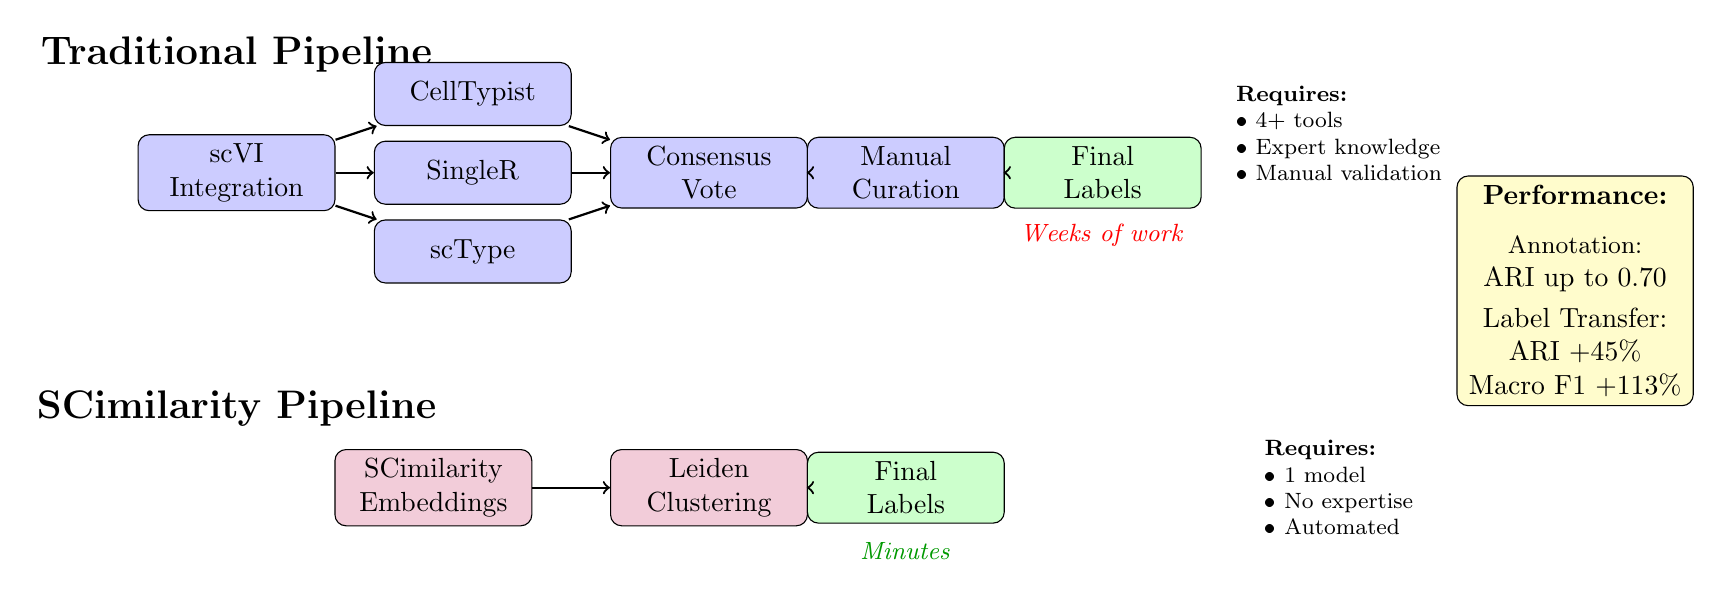
\begin{tikzpicture}[
    node distance=1.5cm,
    box/.style={rectangle, draw, minimum width=2.5cm, minimum height=0.8cm, align=center, rounded corners},
    tool/.style={box, fill=blue!20},
    result/.style={box, fill=green!20},
    scim/.style={box, fill=purple!20},
    arrow/.style={->, thick},
    label/.style={font=\small\bfseries}
]

% Traditional Pipeline (Top)
\node[label] (trad_label) at (-6, 2) {\Large Traditional Pipeline};
\node[tool] (scvi) at (-6, 0.5) {scVI\\Integration};
\node[tool] (celltyp) at (-3, 1.5) {CellTypist};
\node[tool] (singler) at (-3, 0.5) {SingleR};
\node[tool] (sctype) at (-3, -0.5) {scType};
\node[tool] (consensus) at (0, 0.5) {Consensus\\Vote};
\node[tool] (manual) at (2.5, 0.5) {Manual\\Curation};
\node[result] (final_trad) at (5, 0.5) {Final\\Labels};

% Arrows for traditional
\draw[arrow] (scvi) -- (celltyp);
\draw[arrow] (scvi) -- (singler);
\draw[arrow] (scvi) -- (sctype);
\draw[arrow] (celltyp) -- (consensus);
\draw[arrow] (singler) -- (consensus);
\draw[arrow] (sctype) -- (consensus);
\draw[arrow] (consensus) -- (manual);
\draw[arrow] (manual) -- (final_trad);

% Time annotation for traditional
\node[font=\small, text=red] at (5, -0.3) {\textit{Weeks of work}};

% SCimilarity Pipeline (Bottom)
\node[label] (scim_label) at (-6, -2.5) {\Large SCimilarity Pipeline};
\node[scim] (scim_emb) at (-3.5, -3.5) {SCimilarity\\Embeddings};
\node[scim] (leiden) at (0, -3.5) {Leiden\\Clustering};
\node[result] (final_scim) at (2.5, -3.5) {Final\\Labels};

% Arrows for SCimilarity
\draw[arrow] (scim_emb) -- (leiden);
\draw[arrow] (leiden) -- (final_scim);

% Time annotation for SCimilarity
\node[font=\small, text=green!60!black] at (2.5, -4.3) {\textit{Minutes}};

% Comparison annotations
\node[font=\footnotesize, align=left] at (8, 1) {
    \textbf{Requires:}\\
    • 4+ tools\\
    • Expert knowledge\\
    • Manual validation
};

\node[font=\footnotesize, align=left] at (8, -3.5) {
    \textbf{Requires:}\\
    • 1 model\\
    • No expertise\\
    • Automated
};

% Performance box
\node[box, fill=yellow!20, minimum width=3cm, minimum height=2cm] at (11, -1) {
    \textbf{Performance:}\\[0.2cm]
    \small
    Annotation:\\
    ARI up to 0.70\\[0.1cm]
    Label Transfer:\\
    ARI +45\%\\
    Macro F1 +113\%
};

\end{tikzpicture}
\caption{Pipeline comparison for AML cell type annotation. \textbf{Top:} Traditional approach requiring scVI integration, consensus annotation from three tools (CellTypist, SingleR, scType), and extensive manual curation. \textbf{Bottom:} SCimilarity approach using only pre-trained embeddings and simple clustering. Despite dramatically reduced complexity, SCimilarity achieves comparable annotation accuracy (ARI=0.70) and superior label transfer performance, particularly for rare cell types (+113\% macro F1).}
\label{fig:pipeline}
\end{figure}
